
\pdfminorversion=4





\documentclass[11pt]{article}
\usepackage{amsmath, amsthm}
\usepackage[pdftex]{graphicx}
\usepackage{psfrag,epsf}
\usepackage{enumerate}
\usepackage{natbib}
\usepackage{float}
\restylefloat{table}

\usepackage{amssymb}
\usepackage{multirow}
\usepackage{float}
\newtheorem{thm}{Theorem}

\newcommand{\blind}{0}

\addtolength{\oddsidemargin}{-.75in}%
\addtolength{\evensidemargin}{-.75in}%
\addtolength{\textwidth}{1.5in}%
\addtolength{\textheight}{1.3in}%
\addtolength{\topmargin}{-.8in}%

\newtheorem{theorem}{\bf Theorem}
\newtheorem{proposition}{\bf Proposition}
\newtheorem{lemma}{\bf Lemma}
\newtheorem{corollary}{\bf Corollary}
\numberwithin{equation}{section}

\date{\textbf{Draft} \textbf{\today}}
\begin{document}

%\bibliographystyle{natbib}

%\newcommand{\keywords}[1]{\par\addvspace\baselineskip
%\noindent\keywordname\enspace\ignorespaces#1}

\def\spacingset#1{\renewcommand{\baselinestretch}%
{#1}\small\normalsize} \spacingset{1}


%%%%%%%%%%%%%%%%%%%%%%%%%%%%%%%%%%%%%%%%%%%%%%%%%%%%%%%%%%%%%%%%%%%%%%%%%%%%%%

\if0\blind
{
  \title{The Cox Proportional Hazard Model with a Log Concave Baseline with Application to Interval Censored Data}
  \author{Clifford Anderson-Bergman\\
    Department of Statistics, University of California Berkeley\\
    }
  \maketitle
} \fi

\if1\blind
{
  \bigskip
  \bigskip
  \bigskip
  \begin{center}
    {\large\bf The Cox Proportional Hazard Model with a Log Concave Baseline with Application to Interval Censored Data}
\end{center}
  \medskip
} \fi


\spacingset{1.4}


\begin{abstract}

	The Cox Proportional Hazards model is a very popular regression model in the survival analysis setting. For interval censored data, the regression coefficients cannot be estimated independently of the baseline distribution, unlike the case for right censored data. To allow for robust estimation for interval censored data, a common regression model is a Cox Proportional Hazard model where the baseline distribution is estimated with the NPMLE. While this does provide for asymptotically efficient estimation of the regression coefficients, 
the NPMLE has a notoriously slow convergence rate and thus estimates directly involving the baseline survival function will be inefficient. 

	We purpose a Cox Proportional Hazards model in which the baseline distribution is constrained to be log-concave. This provides for more flexibility than a fully parametric model but more efficiency with regards to estimation of the baseline distribution than the NPMLE. We discuss an issue regarding the existence of the maximum likelihood estimate and provide a justified solution that involves augmenting the baseline log concave estimate. We provide an algorithm for computing the Cox Proportional Hazard with baseline log concave estimator. We apply the estimator to simulated data and compare results with competing estimators. Finally, we use our new estimator on a classic dataset comparing rates of lung cancer among RFM mice. 

\end{abstract}

 {\bf Keywords}: Non-parametric, Shape Constraints, Cox PH, Log Concave

{\section{Introduction}  
\label{sec:Intro}	}			
	 	 
	For univariate interval censored data, the non-parametric maximum likelihood estimator (NPMLE) is typically the estimator of choice (Turnbull 1976). The reason for this is that inspecting model fit for parametric models can very difficult with interval censored data and improper model selection can lead to heavy bias. However, the NPMLE has a notorious slow rate of convergence ($n^{-1/3}$ for case I interval censored data, $\log(n) n^{-1/3}$ for case II interval censored data, Gentleman and Vandal ???). In a compromise between flexibility and efficiency, it has been purposed to use a non-parametric maximum likelihood estimator, constrained to have a log-concave density function (Anderson-Bergman and Yu 2014). In addition to providing non-degenerate density estimates, it was found empirically that this improves the rate of convergence, observed from $n^{-2/5}$ to $n^{-1/2}$ in different settings. 

	In the regression setting, one of the most common models for interval censored data is the Cox proportional hazards model. In the case of right censored data, this model is quite popular because the regression coefficients can be estimated independently of the baseline distribution by using only the ordering of the observed times. For interval censored data, this is not the case, as the ordering is often not known due to censoring. However, this model is still popular and is often paired with the unconstrained NPMLE as the baseline survival estimate to provide for a flexible semi parametric estimator. Despite the slow convergence of the NPMLE, the convergence of the regression parameters have been shown to have the more standard $n^{-1/2}$ rate. While this does provide for efficient estimation of the regression parameters, estimations directly involving the baseline distribution, such as survival estimates, will be quite inefficient. 
	
	In this work, we address the problem by constraining the baseline distribution to be log-concave. This leads to a more efficient estimator than the Cox-PH model with the baseline NPMLE, while still being more flexible than a fully parametric model. In section \ref{sec:Naive}, we first introduce the ``naive" likelihood function. We demonstrate how the likelihood function can be unbounded in common situations. In section \ref{sec:Augment} we provide and justify an augmented baseline distribution for which the likelihood will be bounded under minimal conditions. 
		 
{\section{The Naive Likelihood Function} 
\label{sec:Naive}	}				

	The ``naive" log likelihood function would simply involve a baseline log concave density function with the contribution of each observation to the log likelihood function adjusted by the Cox proportional hazards regression estimates. Using the standard interval censored notation, this could be written in the form of 

\[
	\displaystyle \sum_{i = 1}^{n_1} \log (f_0(t_i) \times \eta_i \times S_0(t_i)^{\eta_i - 1})  +
	\displaystyle \sum_{j = 1}^{n_2} \log( S_0( l_j )^{\eta_j} - S_0({r_j})^{\eta_j} ) 
\]	
\[
	f_0 \text{ constrained to be log concave}
\]
	
	where $n_1$ is the number of uncensored observations, $n_2$ is the number of censored observations, $t_i$ is the event time for uncensored subject $i$, $l_j$ and $r_j$ are the left and right sides of the censoring interval for censored subject $j$, $\eta_i = \mathrm{exp}(X_i^t \beta)$, $f_0$ is the baseline distribution and $S_0(t)$ = $\int_t^\infty f_0(s) ds$.
	
	However, in some standard scenarios this function will be unbounded. Consider the case with no censored data. Now the likelihood function can be simplified to 
	
	\[
	\displaystyle \sum_{i = 1}^n \log (f_0(t_i) \times \eta_i \times S_0(t_i)^{\eta_i - 1} ) 
	\]
	
	To heuristically demonstrate the problem, those familiar with the univariate log concave NPMLE (see Rufibach et al ?????) will recognize the maximum likelihood estimator places 0 probability mass beyond $t_{max}$, where $t_{max}$ is the maximum time observed. However, because the Cox PH density at a given point is based on the baseline survival at that point, if 0 probability mass is placed beyond $t_{max}$ then $S_0(t_{max}) = 0$. If $\eta_i < 1$, $f_0(t_{max}) > 0$ and $S_0(t_{max}) = 0$, then the density function will be unbounded as $t \rightarrow t_{max}$  because the log concave constraint will force $f_0$ and $S_0$ to be continuous. This is similar to the issue that for uncensored data, the estimated hazard at $t_{max}$ will always be $\infty$ for the univariate logconcave NPMLE. A more formal proof of this issue can be found in the appendix. 
	
	It is worth noting that in the case where all the data is censored, this does not create an issue with calculation of the likelihood function, as $\hat S_0(t_{max})^{\eta_i} = 0^{\eta_i}=0 $. In the case of both censored and uncensored data, it is uncertain when this will create a problem. In fact, in certain scenarios it will be unknown whether this will create a problem before an optimization algorithm is run. For example, if the data contains a uncensored observation, contained within the interval of censored observation, then it is uncertain whether the estimator will place probability mass to the right of the uncensored observation. 
	
	In order to prevent these potential issues, we purpose an augmenting the log concave estimator to create an estimator $\hat f_{aug}$ such that $\hat f_{aug}(t) > 0$ for $t \in [0, \infty)$. In the next section, we justify use of this augmented estimator. 
	
{\section{Augmenting the Baseline Distribution} 
\label{sec:Augment}} 

	To explore the problem further, we consider three scenarios. 
	
	\begin{itemize}
	
	\item 1.) All the data is uncensored
	
	\item 2.) There exists both censored and uncensored data and $t_{\max}$ (largest uncensored observation) $> l_{\max}$ (largest left side of a censored interval)
	
	\item 3.) There exists both censored and uncensored data and $t_{\max} < l_{\max}$. 
	
	\end{itemize}
	
	In regards to the Cox-PH model with a log-concave baseline, using the ``naive" log concave baseline estimator will lead to ill-defined coefficient estimates in scenarios 1 and 2. This will be fixed by augmenting the estimator which is easily justified in these cases, as we will show shortly. On the other hand, in scenario 3, the ``naive" estimator will lead to valid estimation. However, in some cases we will not be able to distinguish between cases 2 and 3 before an optimization algorithm has been ran. 
	
	With this in mind, we created a single unifying augmentation which provides valid inference for a Cox PH model in all three scenarios. In scenario 1, it is very easy to find a justified amount to augment the estimator by, but in cases 2 and 3, we merely present a lower bound for the amount of augmentation. 
	
	{\subsection{Justification for Augmented}} 
	
	For uncensored data, the crux of the issue with the ``naive" baseline distribution is that the log concave estimator places zero mass beyond $t_{\max}$ for uncensored data (it also places zero mass before $t_{min}$,  which will be addressed but is not a problem for the Cox PH model). This is not a favorable characteristic of the estimator as we typically think of survival functions having positive value on the non-negative real line, and so it makes sense to augment the log concave estimator by forcing mass below $t_{min}$ and above $t_{max}$. In the case of the univariate estimator with uncensored data, the expected value of $F(t_{min})$ and $F(t_{max})$ are $\frac{1}{2n}$ and $\frac{2n-1}{2n}$ respectively, where $F$ is the cdf from which each unordered $t_i$ was drawn. Because of this, it seems reasonable to constrain the log concave estimator to only assign $\frac{n-1}{n}$ probability between $t_{min}$ and $t_{max}$ and then assign $\frac{1}{2n}$ to either side. In addition, if $t_{min} = 0$ was observed, we may opt to assign $\frac{2n-1}{2n}$ between $t_{min}$ and $t_{max}$ and only assign $\frac{1}{2n}$ beyond $t_{max}$. How the augmented probability mass should be assigned is not entirely obvious, although a natural choice for the log-concave estimator is log-linear. 
	
	We note that this is very similar in spirit to using $\hat s = \hat \sigma \sqrt{\frac{n}{n-1}}$ to estimate the standard deviation, where $\hat \sigma$ is the MLE estimate of $\sigma$. 
	
	In the case of univariate data, the augmented estimator can be calculated in closed form the standard log concave estimator, so no new software is required. The density estimates of the augmented estimator can be written as 
	
	\[
	\hat f_{aug}(t) = \hat f_{lc}(t) \times \left(\frac{n-1}{n} \right); t \in [t_{min}, t_{max}]
	\]
	\[
	\hat S_{aug}(t) = \hat S_{lc}(t) \times \left( \frac{n-1}{n}  \right) + \frac{1}{2n}; t \in [t_{min}, t_{max}]
	\]
	
	How the estimator is defined outside of $[t_{min}, t_{max}]$ depends on how the investigator choices to distribute the remaining probability. It can be easily shown that these estimates maximize the likelihood function for univariate (censored or uncensored data) under the constraints that $f_{aug}$ is log-concave on $[t_{min}, t_{max}]$ and $\int_{t_{min}}^{t_{max}} f_{aug}(s) ds = \frac{n-1}{n}$. See appendix for proof. 
	
	To demonstrate the effect this augmentation has on the estimated hazard, we simulated $n = 250$ samples from a exponential(1) distribution and plotted both the estimated hazard function from the standard log concave estimator and from an augmented log concave estimator. Examining figure \ref{fig:AugHaz}, we see that this provides for much more reasonable estimate of the hazard function, specifically as $t$ increases. 
	
	
	\begin{figure}[H]
	\centerline{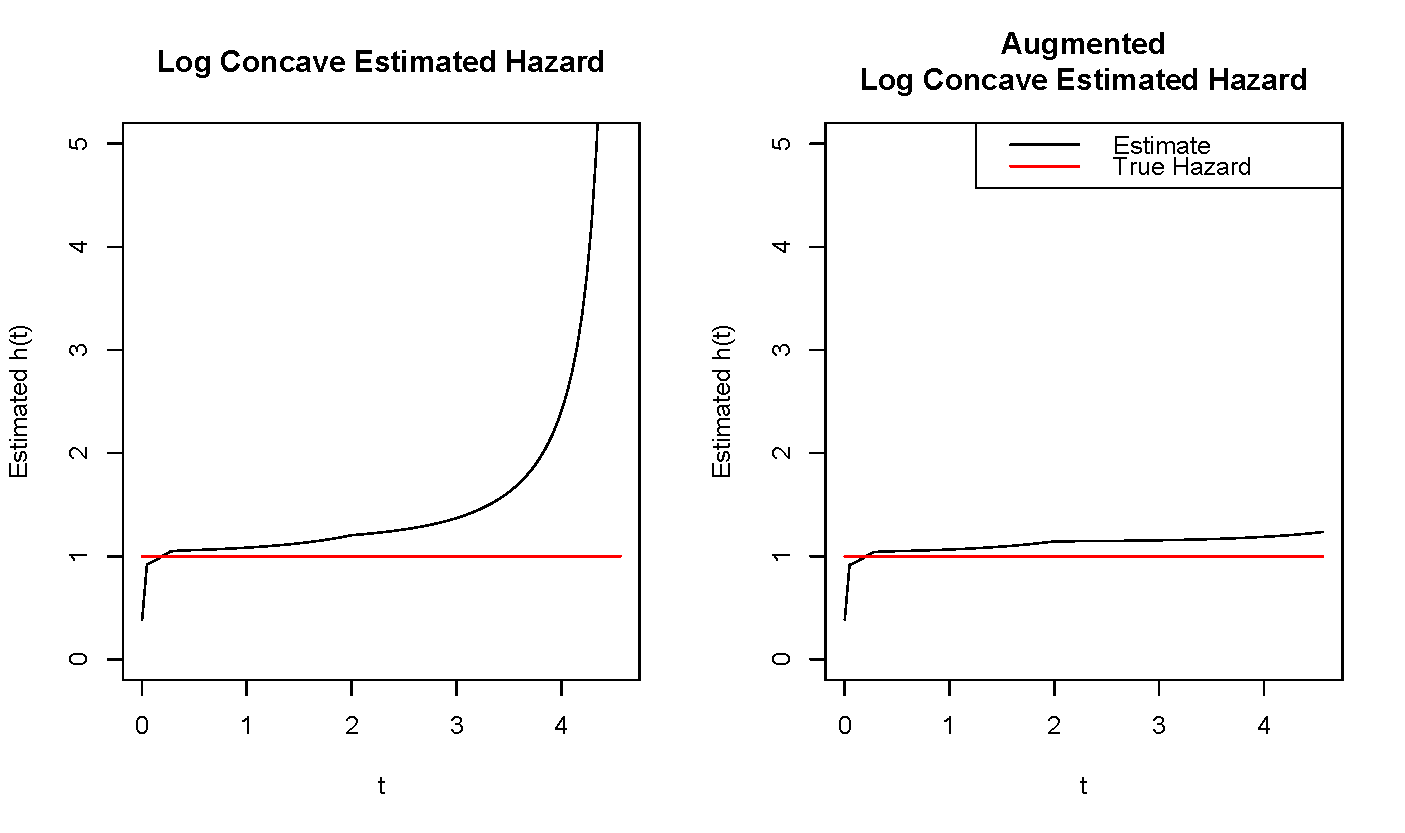
\includegraphics[width = 15cm]{EstimateHazards.pdf} }
	\caption{Estimated Hazard Functions Based on $n = 250$ Simulated Uncensored Exponential(1) Random Variables}
	\label{fig:AugHaz}
	\end{figure} 
	
	When the data contains censored values, we will use the interval censored notation that $l_i$ is the left hand side of the interval and $r_i$ is the right hand side of the interval for subject $i$ and $t^*_i$ refers to the (potentially censored) event time. So although $t^*_i$ may not be known, we do know $t^*_i \in [l_i, r_i]$. Note that uncensored data can be represented as $l_i = r_i = t^*_i$. Under this scheme, the largest confirmed event time (i.e. time when \emph{at least} one event has occurred by) is max($l_i$) and the minimum confirmed event time is min($r_i$). 
	
	Because $t^*_i \in [l_i, r_i]$, we know $\text{max}(t^*_i) \geq \text{max}(l_i)$ and $\text{min}(t^*_i) \leq \text{min}(r_i)$. Therefore,
		
	\[
	\mathbb{E}[F(\max(r_i))] \geq \mathbb{E}[F(t^*_{min})] = \frac{1}{2(n_1 + n_2)}
	\]
	\[
	\mathbb{E}[F(\min(l_i) )] \leq \mathbb{E}[F(t_{max} )] = \frac{2(n_1 + n_2)-1}{2(n_1 +n_2)}
	\]
	
	From this, it seems reasonable to enforce that probability mass $\frac{1}{2n}$ be assigned below $\min(r_i)$ and above $\max(l_i)$. This creates a single well justified rule which can be applied to all scenarios  and prevents the issue of $\hat S(t_{max}) = 0$. 
		
{\section{Augmented Log Likelihood} }
			
	Under this new scheme, the augmented log likelihood can be written as 		
			
\[
	\displaystyle \sum_{i = 1}^{n_1} \log (f_0(t_i) \times \eta_i \times S_0(t_i)^{\eta_i - 1})  +
	\displaystyle \sum_{j = 1}^{n_2} \log( S_0( l_j )^{\eta_j} - S_0({r_j})^{\eta_j} ) 
\]	
\[
	f_0 \text{ constrained to be log concave}
\]
\[
	S_0( r_{min}) \le \frac{2n-1}{2n}
\]			
\[
	S_0( l_{max} ) \ge \frac{1}{2n} 
\]

	where $r_{min} = \min(t_i, r_j)$ and $l_{max} = \max(t_i, l_j)$. All other notation remains the same as in the naive likelihood function. 

{\section{Sufficient Parameter Space}}


{\section{Algorithm} }
		
	To compute the Cox PH model with log concave baseline, a two step algorithm was created. One step updates the regression parameters and one step updates the baseline log concave distribution. To update the regression parameters, Newton's method was used. For the baseline distribution, a sequential 
		
{\section{Conclusion} }

{\section{Appendix}}
 
 \end{document}
	